\section*{Before You Begin}
Welcome to the first assignment of XCS224N! Please note that the core Assignment 1 (not including the Extra Credit which is presented separately) is divided into two tasks:
\begin{enumerate}
    \item A coding assignment in which you will implement a co-occurrence based word embedding model.
    \item A Google CoLab notebook in which you will experiment with pre-trained Word2Vec embeddings, using the results of these experiments to pass a multiple choice quiz. We recommend opening the notebook in a Google Chrome browser.
\end{enumerate}
We highly recommend that you complete these two tasks in order (Part 1 before Part 2). 
\newline

\section*{Word Embeddings (Refresher)}
Presented below is a quick review on word embeddings and their role in NLP. Word Vectors are often used as a fundamental component for downstream NLP tasks, e.g. question answering, text generation, translation, etc., so it is important to build some intuitions as to their strengths and weaknesses. Here you will explore two types of word vectors: those derived from co-occurrence matrices (following section), and those derived via word2vec (last section). In this refresher, we will focus more intently on the details of count-based (co-occurrence) embeddings. \newline

\textbf{Note on Terminology}: The terms ``word vector'' and ``word embedding'' are often used interchangeably. The term ``embedding'' refers to the fact that we are encoding aspects of a word's meaning in a lower dimensional space. As Wikipedia states, ``conceptually it involves a mathematical embedding from a space with one dimension per word to a continuous vector space with a much lower dimension''.

\subsection{Count-Based Word Vectors (Co-occurence)}

A co-occurrence matrix counts how often things co-occur in some environment. Given some word $w_i$ occurring in the document, we consider the \textit{context window} surrounding $w_i$. Supposing our fixed window size is $n$, then this is the $n$ preceding and  $n$ subsequent words in that document, i.e. words  $w_{i-n} \dots w_{i-1}$ and $w_{i+1} \dots w_{i+n}$. We build a co-occurrence matrix $\textbf{M}$, which is a symmetric word-by-word matrix in which $\textbf{M}_{ij}$ is the number of times  $w_{j}$ appears inside $w_{i}$'s window. We provide an example of such a matrix $\textbf{M}$ with window-size $n=1$ for the mock documents below:\newline

Document 1: ``all that glitters is not gold''\newline
Document 2: ``all is well that ends well'' \newline

\begin{equation*}
\textbf{M} = \bordermatrix{& \text{START} & \text{all}& \text{that}& \text{glitters}& \text{is} & \text{not} & \text{gold} & \text{well} & \text{ends} & \text{END}\cr
                \text{START} & 0 & 2 & 0 & 0 & 0 & 0 & 0 & 0 & 0 & 0 \cr
                \text{all} & 2 & 0 & 1 & 0 & 1 & 0 & 0 & 0 & 0 & 0 \cr
                \text{that}& 0 & 1 & 0 & 1 & 0 & 0 & 0 & 1 & 1 & 0 \cr
                \text{glitters}& 0 & 0 & 1 & 0 & 1 & 0 & 0 & 0 & 0 & 0 \cr
                \text{is}& 0 & 1 & 0 & 1 & 0 & 1 & 0 & 1 & 0 & 0 \cr
                \text{not}& 0 & 0 & 0 & 0 & 1 & 0 & 1 & 0 & 0 & 0 \cr
                \text{gold}& 0 & 0 & 0 & 0 & 0 & 1 & 0 & 0 & 0 & 1 \cr
                \text{well}& 0 & 0 & 1 & 0 & 1 & 0 & 0 & 0 & 1 & 1\cr
                \text{ends}& 0 & 0 & 1 & 0 & 0 & 0 & 0 & 1 & 0 & 0\cr
                \text{END}& 0 & 0 & 0 & 0 & 0 & 0 & 1 & 1 & 0 & 0\cr
                }
\end{equation*}
\vspace{15pt}

\textbf{Note}: In NLP, we often add START and END tokens to represent the beginning and end of sentences, paragraphs or documents. In this case we imagine START and END tokens encapsulating each document, e.g., "START All that glitters is not gold END", and include these tokens in our co-occurrence counts.\newline

The rows (or columns) of this matrix provide one type of word vector (those based on word-word co-occurrence), but the vectors will be large in general (linear in the number of distinct words in a corpus). Thus, our next step is to run \textit{dimensionality reduction}. In particular, we will run \textit{SVD (Singular Value Decomposition)}, which is a kind of generalized \textit{PCA (Principal Components Analysis)} to select the top  $k$ principal components. Figure \ref{fig:svd} provides a visualization of dimensionality reduction using SVD. In this picture our co-occurrence matrix is $\textbf{A}$ with $n$ rows corresponding to $n$ words. We obtain a full matrix decomposition, with the singular values ordered in the diagonal $\textbf{S}$ matrix, and our new, shorter-length-$k$ word vectors in $\textbf{U}_k$. 

\begin{figure}[h]
    \centering
    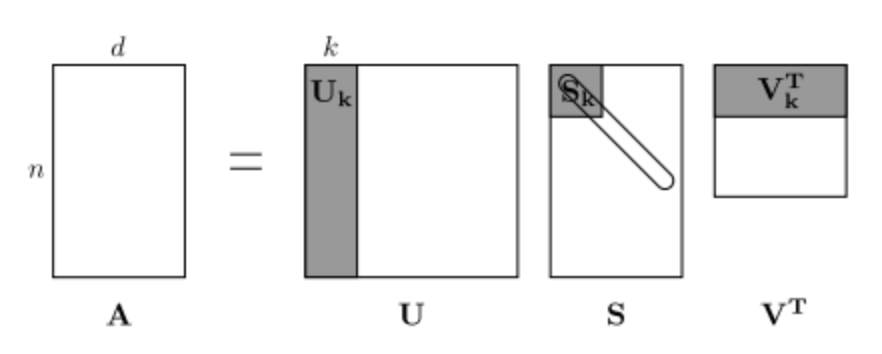
\includegraphics[width=0.5\textwidth]{svd.png}
    \caption{Dimensionality reduction by truncated SVD}
    \label{fig:svd}
\end{figure}

This reduced-dimensionality co-occurrence representation preserves semantic relationships between words, e.g. doctor and hospital will be closer than doctor and dog. \newline

Those interested in getting a deeper mathematical understanding of dimensionality reduction should complete the Extra Credit homework assignment. A slow, friendly introduction to SVD can be found here: \url{https://davetang.org/file/Singular_Value_Decomposition_Tutorial.pdf}. Alternatively, the SVD is a commonly discussed mathematical concept, and a quick Google search will yield a number of valuable resources! 
